\documentclass[1p]{elsarticle_modified}
%\bibliographystyle{elsarticle-num}

%\usepackage[colorlinks]{hyperref}
%\usepackage{abbrmath_seonhwa} %\Abb, \Ascr, \Acal ,\Abf, \Afrak
\usepackage{amsfonts}
\usepackage{amssymb}
\usepackage{amsmath}
\usepackage{amsthm}
\usepackage{scalefnt}
\usepackage{amsbsy}
\usepackage{kotex}
\usepackage{caption}
\usepackage{subfig}
\usepackage{color}
\usepackage{graphicx}
\usepackage{xcolor} %% white, black, red, green, blue, cyan, magenta, yellow
\usepackage{float}
\usepackage{setspace}
\usepackage{hyperref}

\usepackage{tikz}
\usetikzlibrary{arrows}

\usepackage{multirow}
\usepackage{array} % fixed length table
\usepackage{hhline}

%%%%%%%%%%%%%%%%%%%%%
\makeatletter
\renewcommand*\env@matrix[1][\arraystretch]{%
	\edef\arraystretch{#1}%
	\hskip -\arraycolsep
	\let\@ifnextchar\new@ifnextchar
	\array{*\c@MaxMatrixCols c}}
\makeatother %https://tex.stackexchange.com/questions/14071/how-can-i-increase-the-line-spacing-in-a-matrix
%%%%%%%%%%%%%%%

\usepackage[normalem]{ulem}

\newcommand{\msout}[1]{\ifmmode\text{\sout{\ensuremath{#1}}}\else\sout{#1}\fi}
%SOURCE: \msout is \stkout macro in https://tex.stackexchange.com/questions/20609/strikeout-in-math-mode

\newcommand{\cancel}[1]{
	\ifmmode
	{\color{red}\msout{#1}}
	\else
	{\color{red}\sout{#1}}
	\fi
}

\newcommand{\add}[1]{
	{\color{blue}\uwave{#1}}
}

\newcommand{\replace}[2]{
	\ifmmode
	{\color{red}\msout{#1}}{\color{blue}\uwave{#2}}
	\else
	{\color{red}\sout{#1}}{\color{blue}\uwave{#2}}
	\fi
}

\newcommand{\Sol}{\mathcal{S}} %segment
\newcommand{\D}{D} %diagram
\newcommand{\A}{\mathcal{A}} %arc


%%%%%%%%%%%%%%%%%%%%%%%%%%%%%5 test

\def\sl{\operatorname{\textup{SL}}(2,\Cbb)}
\def\psl{\operatorname{\textup{PSL}}(2,\Cbb)}
\def\quan{\mkern 1mu \triangleright \mkern 1mu}

\theoremstyle{definition}
\newtheorem{thm}{Theorem}[section]
\newtheorem{prop}[thm]{Proposition}
\newtheorem{lem}[thm]{Lemma}
\newtheorem{ques}[thm]{Question}
\newtheorem{cor}[thm]{Corollary}
\newtheorem{defn}[thm]{Definition}
\newtheorem{exam}[thm]{Example}
\newtheorem{rmk}[thm]{Remark}
\newtheorem{alg}[thm]{Algorithm}

\newcommand{\I}{\sqrt{-1}}
\begin{document}

%\begin{frontmatter}
%
%\title{Boundary parabolic representations of knots up to 8 crossings}
%
%%% Group authors per affiliation:
%\author{Yunhi Cho} 
%\address{Department of Mathematics, University of Seoul, Seoul, Korea}
%\ead{yhcho@uos.ac.kr}
%
%
%\author{Seonhwa Kim} %\fnref{s_kim}}
%\address{Center for Geometry and Physics, Institute for Basic Science, Pohang, 37673, Korea}
%\ead{ryeona17@ibs.re.kr}
%
%\author{Hyuk Kim}
%\address{Department of Mathematical Sciences, Seoul National University, Seoul 08826, Korea}
%\ead{hyukkim@snu.ac.kr}
%
%\author{Seokbeom Yoon}
%\address{Department of Mathematical Sciences, Seoul National University, Seoul, 08826,  Korea}
%\ead{sbyoon15@snu.ac.kr}
%
%\begin{abstract}
%We find all boundary parabolic representation of knots up to 8 crossings.
%
%\end{abstract}
%\begin{keyword}
%    \MSC[2010] 57M25 
%\end{keyword}
%
%\end{frontmatter}

%\linenumbers
%\tableofcontents
%
\newcommand\colored[1]{\textcolor{white}{\rule[-0.35ex]{0.8em}{1.4ex}}\kern-0.8em\color{red} #1}%
%\newcommand\colored[1]{\textcolor{white}{ #1}\kern-2.17ex	\textcolor{white}{ #1}\kern-1.81ex	\textcolor{white}{ #1}\kern-2.15ex\color{red}#1	}

{\Large $\underline{12n_{0018}~(K12n_{0018})}$}

\setlength{\tabcolsep}{10pt}
\renewcommand{\arraystretch}{1.6}
\vspace{1cm}\begin{tabular}{m{100pt}>{\centering\arraybackslash}m{274pt}}
\multirow{5}{120pt}{
	\centering
	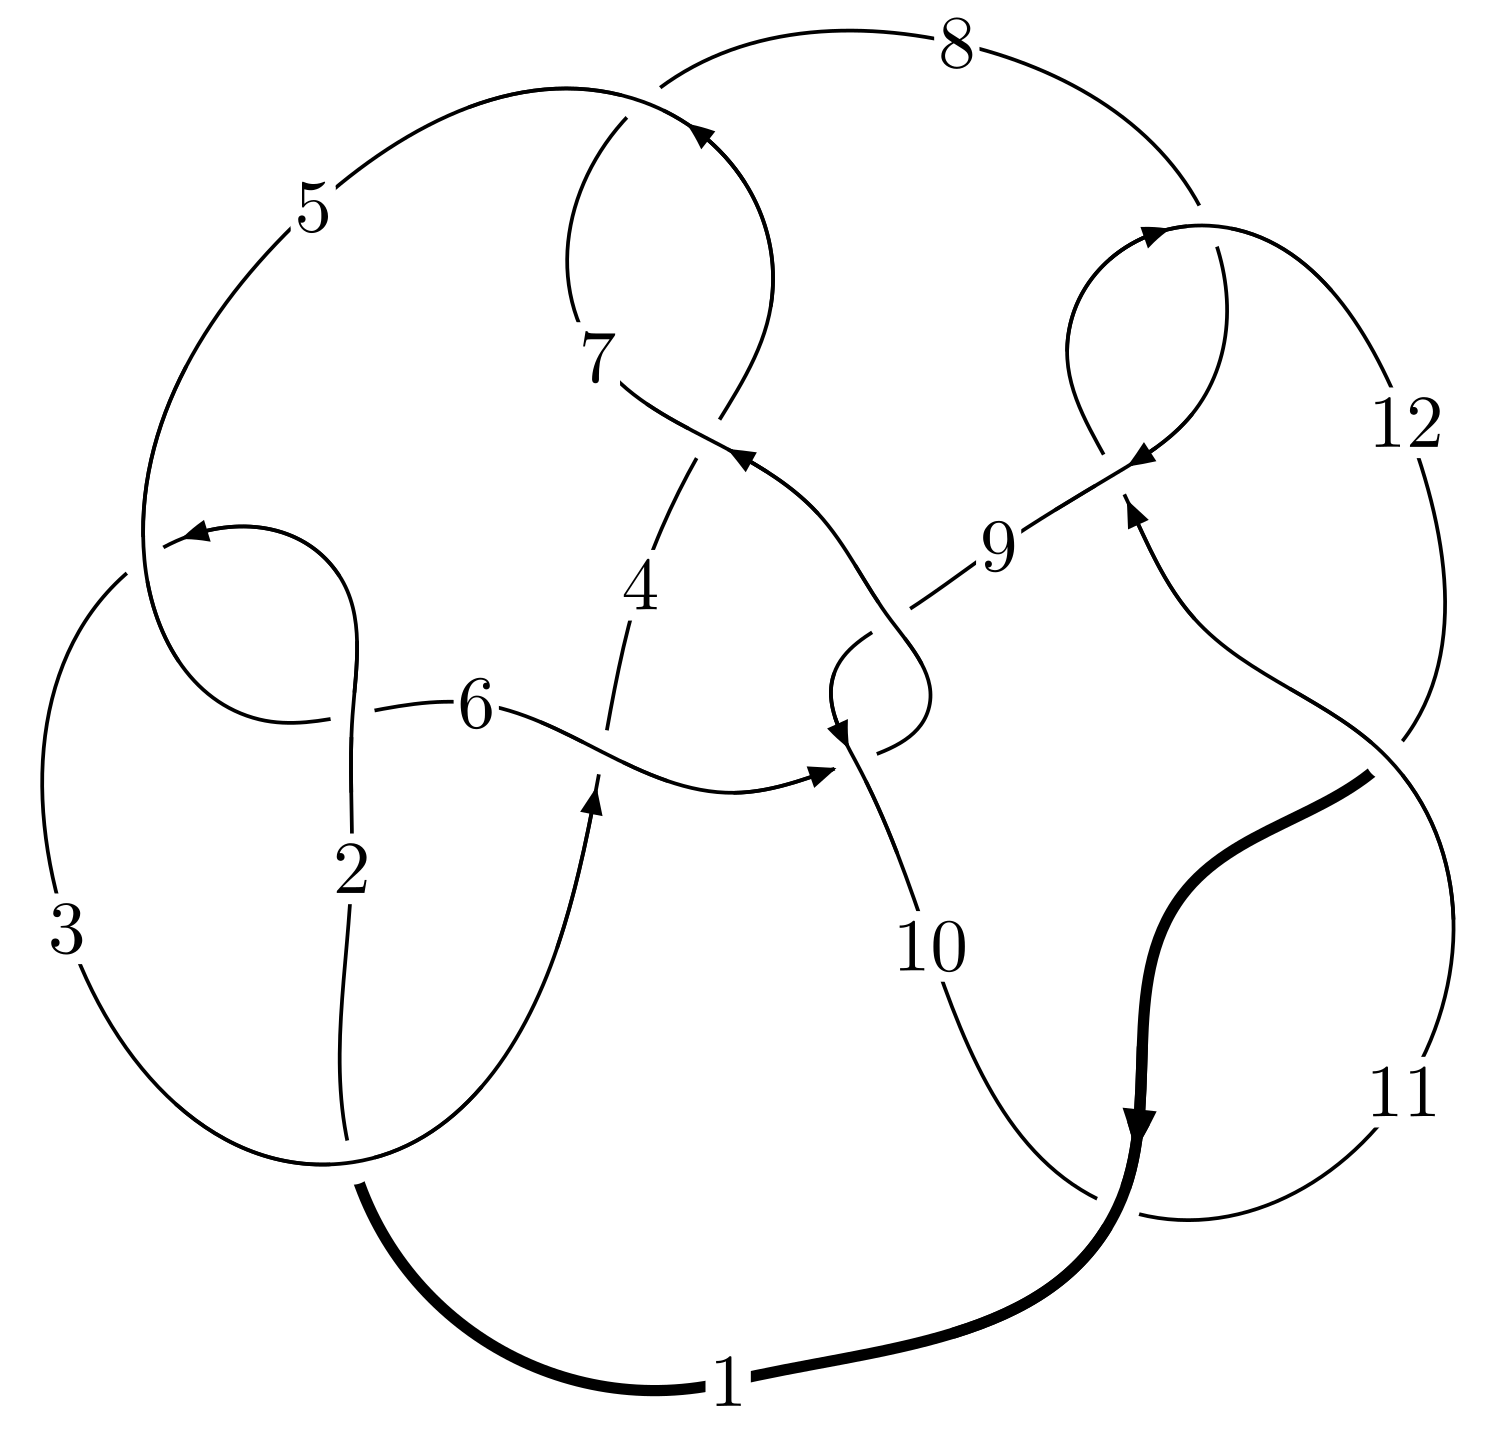
\includegraphics[width=112pt]{../../../GIT/diagram.site/Diagrams/png/2107_12n_0018.png}\\
\ \ \ A knot diagram\footnotemark}&
\allowdisplaybreaks
\textbf{Linearized knot diagam} \\
\cline{2-2}
 &
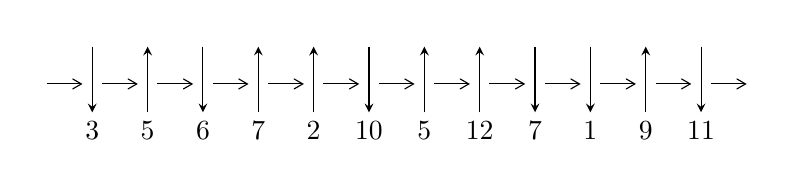
\begin{tikzpicture}[x=20pt, y=17pt]
	% nodes
	\node (C0) at (0, 0) {};
	\node (C1) at (1, 0) {};
	\node (C1U) at (1, +1) {};
	\node (C1D) at (1, -1) {3};

	\node (C2) at (2, 0) {};
	\node (C2U) at (2, +1) {};
	\node (C2D) at (2, -1) {5};

	\node (C3) at (3, 0) {};
	\node (C3U) at (3, +1) {};
	\node (C3D) at (3, -1) {6};

	\node (C4) at (4, 0) {};
	\node (C4U) at (4, +1) {};
	\node (C4D) at (4, -1) {7};

	\node (C5) at (5, 0) {};
	\node (C5U) at (5, +1) {};
	\node (C5D) at (5, -1) {2};

	\node (C6) at (6, 0) {};
	\node (C6U) at (6, +1) {};
	\node (C6D) at (6, -1) {10};

	\node (C7) at (7, 0) {};
	\node (C7U) at (7, +1) {};
	\node (C7D) at (7, -1) {5};

	\node (C8) at (8, 0) {};
	\node (C8U) at (8, +1) {};
	\node (C8D) at (8, -1) {12};

	\node (C9) at (9, 0) {};
	\node (C9U) at (9, +1) {};
	\node (C9D) at (9, -1) {7};

	\node (C10) at (10, 0) {};
	\node (C10U) at (10, +1) {};
	\node (C10D) at (10, -1) {1};

	\node (C11) at (11, 0) {};
	\node (C11U) at (11, +1) {};
	\node (C11D) at (11, -1) {9};

	\node (C12) at (12, 0) {};
	\node (C12U) at (12, +1) {};
	\node (C12D) at (12, -1) {11};
	\node (C13) at (13, 0) {};

	% arrows
	\draw[->,>={angle 60}]
	(C0) edge (C1) (C1) edge (C2) (C2) edge (C3) (C3) edge (C4) (C4) edge (C5) (C5) edge (C6) (C6) edge (C7) (C7) edge (C8) (C8) edge (C9) (C9) edge (C10) (C10) edge (C11) (C11) edge (C12) (C12) edge (C13) ;	\draw[->,>=stealth]
	(C1U) edge (C1D) (C2D) edge (C2U) (C3U) edge (C3D) (C4D) edge (C4U) (C5D) edge (C5U) (C6U) edge (C6D) (C7D) edge (C7U) (C8D) edge (C8U) (C9U) edge (C9D) (C10U) edge (C10D) (C11D) edge (C11U) (C12U) edge (C12D) ;
	\end{tikzpicture} \\
\hhline{~~} \\& 
\textbf{Solving Sequence} \\ \cline{2-2} 
 &
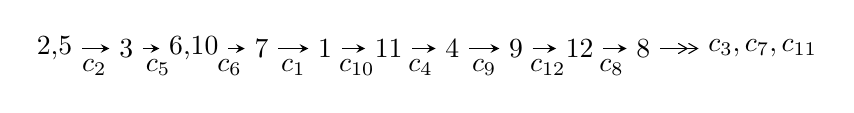
\begin{tikzpicture}[x=23pt, y=7pt]
	% node
	\node (A0) at (-1/8, 0) {2,5};
	\node (A1) at (1, 0) {3};
	\node (A2) at (33/16, 0) {6,10};
	\node (A3) at (25/8, 0) {7};
	\node (A4) at (33/8, 0) {1};
	\node (A5) at (41/8, 0) {11};
	\node (A6) at (49/8, 0) {4};
	\node (A7) at (57/8, 0) {9};
	\node (A8) at (65/8, 0) {12};
	\node (A9) at (73/8, 0) {8};
	\node (C1) at (1/2, -1) {$c_{2}$};
	\node (C2) at (3/2, -1) {$c_{5}$};
	\node (C3) at (21/8, -1) {$c_{6}$};
	\node (C4) at (29/8, -1) {$c_{1}$};
	\node (C5) at (37/8, -1) {$c_{10}$};
	\node (C6) at (45/8, -1) {$c_{4}$};
	\node (C7) at (53/8, -1) {$c_{9}$};
	\node (C8) at (61/8, -1) {$c_{12}$};
	\node (C9) at (69/8, -1) {$c_{8}$};
	\node (A10) at (11, 0) {$c_{3},c_{7},c_{11}$};

	% edge
	\draw[->,>=stealth]	
	(A0) edge (A1) (A1) edge (A2) (A2) edge (A3) (A3) edge (A4) (A4) edge (A5) (A5) edge (A6) (A6) edge (A7) (A7) edge (A8) (A8) edge (A9) ;
	\draw[->>,>={angle 60}]	
	(A9) edge (A10);
\end{tikzpicture} \\ 

\end{tabular} \\

\footnotetext{
The image of knot diagram is generated by the software ``\textbf{Draw programme}" developed by Andrew Bartholomew(\url{http://www.layer8.co.uk/maths/draw/index.htm\#Running-draw}), where we modified some parts for our purpose(\url{https://github.com/CATsTAILs/LinksPainter}).
}\phantom \\ \newline 
\centering \textbf{Ideals for irreducible components\footnotemark of $X_{\text{par}}$} 
 
\begin{align*}
I^u_{1}&=\langle 
2.62383\times10^{39} u^{61}-1.19751\times10^{40} u^{60}+\cdots+3.98732\times10^{38} b-9.31049\times10^{39},\\
\phantom{I^u_{1}}&\phantom{= \langle  }-3.15003\times10^{39} u^{61}+1.51549\times10^{40} u^{60}+\cdots+1.99366\times10^{38} a+1.87829\times10^{40},\\
\phantom{I^u_{1}}&\phantom{= \langle  }u^{62}-5 u^{61}+\cdots-19 u+1\rangle \\
I^u_{2}&=\langle 
a^3 u+a^3-2 a^2-3 a u+b- a+u+1,\;a^4+2 a^3 u-3 a^2 u-3 a^2+a+u,\;u^2+u+1\rangle \\
\\
\end{align*}
\raggedright * 2 irreducible components of $\dim_{\mathbb{C}}=0$, with total 70 representations.\\
\footnotetext{All coefficients of polynomials are rational numbers. But the coefficients are sometimes approximated in decimal forms when there is not enough margin.}
\newpage
\renewcommand{\arraystretch}{1}
\centering \section*{I. $I^u_{1}= \langle 2.62\times10^{39} u^{61}-1.20\times10^{40} u^{60}+\cdots+3.99\times10^{38} b-9.31\times10^{39},\;-3.15\times10^{39} u^{61}+1.52\times10^{40} u^{60}+\cdots+1.99\times10^{38} a+1.88\times10^{40},\;u^{62}-5 u^{61}+\cdots-19 u+1 \rangle$}
\flushleft \textbf{(i) Arc colorings}\\
\begin{tabular}{m{7pt} m{180pt} m{7pt} m{180pt} }
\flushright $a_{2}=$&$\begin{pmatrix}1\\0\end{pmatrix}$ \\
\flushright $a_{5}=$&$\begin{pmatrix}0\\u\end{pmatrix}$ \\
\flushright $a_{3}=$&$\begin{pmatrix}1\\- u^2\end{pmatrix}$ \\
\flushright $a_{6}=$&$\begin{pmatrix}u\\u\end{pmatrix}$ \\
\flushright $a_{10}=$&$\begin{pmatrix}15.8002 u^{61}-76.0156 u^{60}+\cdots+1227.65 u-94.2130\\-6.58044 u^{61}+30.0330 u^{60}+\cdots-304.461 u+23.3502\end{pmatrix}$ \\
\flushright $a_{7}=$&$\begin{pmatrix}-15.9053 u^{61}+77.9924 u^{60}+\cdots-1333.00 u+105.025\\8.30759 u^{61}-33.2844 u^{60}+\cdots+178.838 u-14.4250\end{pmatrix}$ \\
\flushright $a_{1}=$&$\begin{pmatrix}u^2+1\\- u^4\end{pmatrix}$ \\
\flushright $a_{11}=$&$\begin{pmatrix}19.2096 u^{61}-92.8297 u^{60}+\cdots+1541.75 u-118.551\\-8.39084 u^{61}+37.4877 u^{60}+\cdots-309.379 u+23.5628\end{pmatrix}$ \\
\flushright $a_{4}=$&$\begin{pmatrix}u^4+u^2+1\\u^4\end{pmatrix}$ \\
\flushright $a_{9}=$&$\begin{pmatrix}23.0925 u^{61}-111.738 u^{60}+\cdots+1863.68 u-145.752\\-10.1051 u^{61}+43.0078 u^{60}+\cdots-361.476 u+28.7800\end{pmatrix}$ \\
\flushright $a_{12}=$&$\begin{pmatrix}15.5897 u^{61}-75.0040 u^{60}+\cdots+1258.28 u-100.587\\-1.52637 u^{61}+10.2099 u^{60}+\cdots-153.436 u+11.8910\end{pmatrix}$ \\
\flushright $a_{8}=$&$\begin{pmatrix}15.9053 u^{61}-77.9924 u^{60}+\cdots+1333.00 u-105.025\\-10.5447 u^{61}+39.2440 u^{60}+\cdots-192.085 u+15.9594\end{pmatrix}$\\&\end{tabular}
\flushleft \textbf{(ii) Obstruction class $= -1$}\\~\\
\flushleft \textbf{(iii) Cusp Shapes $= 32.0809 u^{61}-157.631 u^{60}+\cdots+2379.84 u-187.341$}\\~\\
\newpage\renewcommand{\arraystretch}{1}
\flushleft \textbf{(iv) u-Polynomials at the component}\newline \\
\begin{tabular}{m{50pt}|m{274pt}}
Crossings & \hspace{64pt}u-Polynomials at each crossing \\
\hline $$\begin{aligned}c_{1}\end{aligned}$$&$\begin{aligned}
&u^{62}+33 u^{61}+\cdots-77 u+1
\end{aligned}$\\
\hline $$\begin{aligned}c_{2},c_{5}\end{aligned}$$&$\begin{aligned}
&u^{62}+5 u^{61}+\cdots+19 u+1
\end{aligned}$\\
\hline $$\begin{aligned}c_{3}\end{aligned}$$&$\begin{aligned}
&u^{62}-5 u^{61}+\cdots+28315 u+1921
\end{aligned}$\\
\hline $$\begin{aligned}c_{4},c_{7}\end{aligned}$$&$\begin{aligned}
&u^{62}+5 u^{61}+\cdots-1152 u+256
\end{aligned}$\\
\hline $$\begin{aligned}c_{6},c_{9}\end{aligned}$$&$\begin{aligned}
&u^{62}-3 u^{61}+\cdots-3 u+1
\end{aligned}$\\
\hline $$\begin{aligned}c_{8},c_{11}\end{aligned}$$&$\begin{aligned}
&u^{62}+3 u^{61}+\cdots-5 u+1
\end{aligned}$\\
\hline $$\begin{aligned}c_{10},c_{12}\end{aligned}$$&$\begin{aligned}
&u^{62}+23 u^{61}+\cdots+11 u+1
\end{aligned}$\\
\hline
\end{tabular}\\~\\
\newpage\renewcommand{\arraystretch}{1}
\flushleft \textbf{(v) Riley Polynomials at the component}\newline \\
\begin{tabular}{m{50pt}|m{274pt}}
Crossings & \hspace{64pt}Riley Polynomials at each crossing \\
\hline $$\begin{aligned}c_{1}\end{aligned}$$&$\begin{aligned}
&y^{62}-3 y^{61}+\cdots-3593 y+1
\end{aligned}$\\
\hline $$\begin{aligned}c_{2},c_{5}\end{aligned}$$&$\begin{aligned}
&y^{62}+33 y^{61}+\cdots-77 y+1
\end{aligned}$\\
\hline $$\begin{aligned}c_{3}\end{aligned}$$&$\begin{aligned}
&y^{62}-39 y^{61}+\cdots-237987197 y+3690241
\end{aligned}$\\
\hline $$\begin{aligned}c_{4},c_{7}\end{aligned}$$&$\begin{aligned}
&y^{62}+45 y^{61}+\cdots+1261568 y+65536
\end{aligned}$\\
\hline $$\begin{aligned}c_{6},c_{9}\end{aligned}$$&$\begin{aligned}
&y^{62}+15 y^{61}+\cdots+11 y+1
\end{aligned}$\\
\hline $$\begin{aligned}c_{8},c_{11}\end{aligned}$$&$\begin{aligned}
&y^{62}+23 y^{61}+\cdots+11 y+1
\end{aligned}$\\
\hline $$\begin{aligned}c_{10},c_{12}\end{aligned}$$&$\begin{aligned}
&y^{62}+35 y^{61}+\cdots-185 y+1
\end{aligned}$\\
\hline
\end{tabular}\\~\\
\newpage\flushleft \textbf{(vi) Complex Volumes and Cusp Shapes}
$$\begin{array}{c|c|c}  
\text{Solutions to }I^u_{1}& \I (\text{vol} + \sqrt{-1}CS) & \text{Cusp shape}\\
 \hline 
\begin{aligned}
u &= \phantom{-}0.965704 + 0.297719 I \\
a &= -1.43043 - 0.52995 I \\
b &= -0.306577 + 0.174570 I\end{aligned}
 & -1.29157 - 10.33450 I & \phantom{-0.000000 } 0 \\ \hline\begin{aligned}
u &= \phantom{-}0.965704 - 0.297719 I \\
a &= -1.43043 + 0.52995 I \\
b &= -0.306577 - 0.174570 I\end{aligned}
 & -1.29157 + 10.33450 I & \phantom{-0.000000 } 0 \\ \hline\begin{aligned}
u &= -0.411885 + 0.945709 I \\
a &= -2.27569 + 1.18972 I \\
b &= -1.71285 + 1.28141 I\end{aligned}
 & -0.55472 - 4.37820 I & \phantom{-0.000000 } 0 \\ \hline\begin{aligned}
u &= -0.411885 - 0.945709 I \\
a &= -2.27569 - 1.18972 I \\
b &= -1.71285 - 1.28141 I\end{aligned}
 & -0.55472 + 4.37820 I & \phantom{-0.000000 } 0 \\ \hline\begin{aligned}
u &= -0.508605 + 0.906380 I \\
a &= \phantom{-}2.86917 - 1.37868 I \\
b &= \phantom{-}2.47102 - 1.51786 I\end{aligned}
 & -0.017864 - 0.355429 I & \phantom{-0.000000 } 0 \\ \hline\begin{aligned}
u &= -0.508605 - 0.906380 I \\
a &= \phantom{-}2.86917 + 1.37868 I \\
b &= \phantom{-}2.47102 + 1.51786 I\end{aligned}
 & -0.017864 + 0.355429 I & \phantom{-0.000000 } 0 \\ \hline\begin{aligned}
u &= \phantom{-}0.892742 + 0.303283 I \\
a &= \phantom{-}1.40786 + 0.50551 I \\
b &= \phantom{-}0.211520 - 0.223149 I\end{aligned}
 & \phantom{-}0.27929 - 4.71522 I & \phantom{-0.000000 } 0 \\ \hline\begin{aligned}
u &= \phantom{-}0.892742 - 0.303283 I \\
a &= \phantom{-}1.40786 - 0.50551 I \\
b &= \phantom{-}0.211520 + 0.223149 I\end{aligned}
 & \phantom{-}0.27929 + 4.71522 I & \phantom{-0.000000 } 0 \\ \hline\begin{aligned}
u &= -0.930590 + 0.096301 I \\
a &= \phantom{-}0.057491 - 0.985327 I \\
b &= -0.005994 - 0.189910 I\end{aligned}
 & \phantom{-}3.48850 - 2.47160 I & \phantom{-}10.13177 + 3.68218 I \\ \hline\begin{aligned}
u &= -0.930590 - 0.096301 I \\
a &= \phantom{-}0.057491 + 0.985327 I \\
b &= -0.005994 + 0.189910 I\end{aligned}
 & \phantom{-}3.48850 + 2.47160 I & \phantom{-}10.13177 - 3.68218 I\\
 \hline 
 \end{array}$$\newpage$$\begin{array}{c|c|c}  
\text{Solutions to }I^u_{1}& \I (\text{vol} + \sqrt{-1}CS) & \text{Cusp shape}\\
 \hline 
\begin{aligned}
u &= \phantom{-}0.374481 + 0.850793 I \\
a &= -0.743628 + 0.575009 I \\
b &= \phantom{-}0.77387 + 1.47048 I\end{aligned}
 & \phantom{-}6.46808 + 4.86140 I & \phantom{-0.000000 } 0 \\ \hline\begin{aligned}
u &= \phantom{-}0.374481 - 0.850793 I \\
a &= -0.743628 - 0.575009 I \\
b &= \phantom{-}0.77387 - 1.47048 I\end{aligned}
 & \phantom{-}6.46808 - 4.86140 I & \phantom{-0.000000 } 0 \\ \hline\begin{aligned}
u &= \phantom{-}0.891739 + 0.124753 I \\
a &= -1.43390 - 0.46536 I \\
b &= -0.330798 + 0.437779 I\end{aligned}
 & -5.82429 - 3.24893 I & -2.83073 + 2.56223 I \\ \hline\begin{aligned}
u &= \phantom{-}0.891739 - 0.124753 I \\
a &= -1.43390 + 0.46536 I \\
b &= -0.330798 - 0.437779 I\end{aligned}
 & -5.82429 + 3.24893 I & -2.83073 - 2.56223 I \\ \hline\begin{aligned}
u &= -0.531933 + 0.965807 I \\
a &= \phantom{-}0.024523 - 1.037090 I \\
b &= \phantom{-}0.21487 - 1.50621 I\end{aligned}
 & -0.14262 - 2.78903 I & \phantom{-0.000000 } 0 \\ \hline\begin{aligned}
u &= -0.531933 - 0.965807 I \\
a &= \phantom{-}0.024523 + 1.037090 I \\
b &= \phantom{-}0.21487 + 1.50621 I\end{aligned}
 & -0.14262 + 2.78903 I & \phantom{-0.000000 } 0 \\ \hline\begin{aligned}
u &= \phantom{-}0.382543 + 0.801832 I \\
a &= \phantom{-}0.843253 - 0.451303 I \\
b &= -0.78761 - 1.22730 I\end{aligned}
 & \phantom{-}6.61497 - 1.56581 I & \phantom{-0.000000 -}0. + 8.95092 I \\ \hline\begin{aligned}
u &= \phantom{-}0.382543 - 0.801832 I \\
a &= \phantom{-}0.843253 + 0.451303 I \\
b &= -0.78761 + 1.22730 I\end{aligned}
 & \phantom{-}6.61497 + 1.56581 I & \phantom{-0.000000 } 0. - 8.95092 I \\ \hline\begin{aligned}
u &= -0.480114 + 0.743056 I \\
a &= \phantom{-}2.00911 - 1.21894 I \\
b &= \phantom{-}1.67487 - 1.75063 I\end{aligned}
 & \phantom{-}0.46926 - 3.71058 I & -6.23280 + 11.34763 I \\ \hline\begin{aligned}
u &= -0.480114 - 0.743056 I \\
a &= \phantom{-}2.00911 + 1.21894 I \\
b &= \phantom{-}1.67487 + 1.75063 I\end{aligned}
 & \phantom{-}0.46926 + 3.71058 I & -6.23280 - 11.34763 I\\
 \hline 
 \end{array}$$\newpage$$\begin{array}{c|c|c}  
\text{Solutions to }I^u_{1}& \I (\text{vol} + \sqrt{-1}CS) & \text{Cusp shape}\\
 \hline 
\begin{aligned}
u &= -0.094130 + 0.841210 I \\
a &= -1.51231 + 1.09297 I \\
b &= -0.499665 + 1.237070 I\end{aligned}
 & -1.62196 + 1.23455 I & -2.69106 - 2.17099 I \\ \hline\begin{aligned}
u &= -0.094130 - 0.841210 I \\
a &= -1.51231 - 1.09297 I \\
b &= -0.499665 - 1.237070 I\end{aligned}
 & -1.62196 - 1.23455 I & -2.69106 + 2.17099 I \\ \hline\begin{aligned}
u &= -0.257077 + 1.145650 I \\
a &= -0.587485 + 0.772224 I \\
b &= -0.87373 + 1.43182 I\end{aligned}
 & -3.22451 - 2.34711 I & \phantom{-0.000000 } 0 \\ \hline\begin{aligned}
u &= -0.257077 - 1.145650 I \\
a &= -0.587485 - 0.772224 I \\
b &= -0.87373 - 1.43182 I\end{aligned}
 & -3.22451 + 2.34711 I & \phantom{-0.000000 } 0 \\ \hline\begin{aligned}
u &= -0.900002 + 0.754167 I \\
a &= \phantom{-}0.124095 - 0.287439 I \\
b &= -0.145127 + 0.264679 I\end{aligned}
 & \phantom{-}2.84220 - 0.80883 I & \phantom{-0.000000 } 0 \\ \hline\begin{aligned}
u &= -0.900002 - 0.754167 I \\
a &= \phantom{-}0.124095 + 0.287439 I \\
b &= -0.145127 - 0.264679 I\end{aligned}
 & \phantom{-}2.84220 + 0.80883 I & \phantom{-0.000000 } 0 \\ \hline\begin{aligned}
u &= -0.475785 + 0.628202 I \\
a &= \phantom{-}1.193400 - 0.639563 I \\
b &= \phantom{-}0.566847 - 0.143962 I\end{aligned}
 & \phantom{-}0.84056 - 1.37461 I & \phantom{-}5.29052 + 4.27881 I \\ \hline\begin{aligned}
u &= -0.475785 - 0.628202 I \\
a &= \phantom{-}1.193400 + 0.639563 I \\
b &= \phantom{-}0.566847 + 0.143962 I\end{aligned}
 & \phantom{-}0.84056 + 1.37461 I & \phantom{-}5.29052 - 4.27881 I \\ \hline\begin{aligned}
u &= \phantom{-}0.442572 + 1.154760 I \\
a &= \phantom{-}0.043171 + 0.738046 I \\
b &= -0.93124 + 1.40738 I\end{aligned}
 & -3.45908 + 2.42252 I & \phantom{-0.000000 } 0 \\ \hline\begin{aligned}
u &= \phantom{-}0.442572 - 1.154760 I \\
a &= \phantom{-}0.043171 - 0.738046 I \\
b &= -0.93124 - 1.40738 I\end{aligned}
 & -3.45908 - 2.42252 I & \phantom{-0.000000 } 0\\
 \hline 
 \end{array}$$\newpage$$\begin{array}{c|c|c}  
\text{Solutions to }I^u_{1}& \I (\text{vol} + \sqrt{-1}CS) & \text{Cusp shape}\\
 \hline 
\begin{aligned}
u &= \phantom{-}0.745927 + 0.110754 I \\
a &= -1.277990 + 0.457571 I \\
b &= -0.255752 - 0.786572 I\end{aligned}
 & -1.84493 - 3.74840 I & \phantom{-}0.35274 + 2.59409 I \\ \hline\begin{aligned}
u &= \phantom{-}0.745927 - 0.110754 I \\
a &= -1.277990 - 0.457571 I \\
b &= -0.255752 + 0.786572 I\end{aligned}
 & -1.84493 + 3.74840 I & \phantom{-}0.35274 - 2.59409 I \\ \hline\begin{aligned}
u &= \phantom{-}0.468807 + 1.155530 I \\
a &= -0.152066 + 1.342220 I \\
b &= \phantom{-}0.48466 + 2.34406 I\end{aligned}
 & -3.26706 + 5.72300 I & \phantom{-0.000000 } 0 \\ \hline\begin{aligned}
u &= \phantom{-}0.468807 - 1.155530 I \\
a &= -0.152066 - 1.342220 I \\
b &= \phantom{-}0.48466 - 2.34406 I\end{aligned}
 & -3.26706 - 5.72300 I & \phantom{-0.000000 } 0 \\ \hline\begin{aligned}
u &= \phantom{-}0.406251 + 1.185420 I \\
a &= \phantom{-}0.29707 - 1.44572 I \\
b &= -0.37469 - 2.34822 I\end{aligned}
 & -5.55349 + 0.20577 I & \phantom{-0.000000 } 0 \\ \hline\begin{aligned}
u &= \phantom{-}0.406251 - 1.185420 I \\
a &= \phantom{-}0.29707 + 1.44572 I \\
b &= -0.37469 + 2.34822 I\end{aligned}
 & -5.55349 - 0.20577 I & \phantom{-0.000000 } 0 \\ \hline\begin{aligned}
u &= -0.893686 + 0.884980 I \\
a &= \phantom{-}0.0151757 + 0.0943643 I \\
b &= \phantom{-}0.275198 - 0.425254 I\end{aligned}
 & \phantom{-}2.47898 - 5.65478 I & \phantom{-0.000000 } 0 \\ \hline\begin{aligned}
u &= -0.893686 - 0.884980 I \\
a &= \phantom{-}0.0151757 - 0.0943643 I \\
b &= \phantom{-}0.275198 + 0.425254 I\end{aligned}
 & \phantom{-}2.47898 + 5.65478 I & \phantom{-0.000000 } 0 \\ \hline\begin{aligned}
u &= \phantom{-}0.236000 + 1.238430 I \\
a &= -0.245273 + 0.777145 I \\
b &= -0.93517 + 1.48259 I\end{aligned}
 & -4.87637 - 1.25419 I & \phantom{-0.000000 } 0 \\ \hline\begin{aligned}
u &= \phantom{-}0.236000 - 1.238430 I \\
a &= -0.245273 - 0.777145 I \\
b &= -0.93517 - 1.48259 I\end{aligned}
 & -4.87637 + 1.25419 I & \phantom{-0.000000 } 0\\
 \hline 
 \end{array}$$\newpage$$\begin{array}{c|c|c}  
\text{Solutions to }I^u_{1}& \I (\text{vol} + \sqrt{-1}CS) & \text{Cusp shape}\\
 \hline 
\begin{aligned}
u &= -0.331100 + 0.640866 I \\
a &= -1.73450 + 0.49909 I \\
b &= -1.35558 + 1.35491 I\end{aligned}
 & \phantom{-}0.414871 + 0.997099 I & -2.34753 + 0.60698 I \\ \hline\begin{aligned}
u &= -0.331100 - 0.640866 I \\
a &= -1.73450 - 0.49909 I \\
b &= -1.35558 - 1.35491 I\end{aligned}
 & \phantom{-}0.414871 - 0.997099 I & -2.34753 - 0.60698 I \\ \hline\begin{aligned}
u &= \phantom{-}0.493150 + 1.180330 I \\
a &= -0.100543 - 0.798998 I \\
b &= \phantom{-}0.89247 - 1.38242 I\end{aligned}
 & -4.93269 + 8.34798 I & \phantom{-0.000000 } 0 \\ \hline\begin{aligned}
u &= \phantom{-}0.493150 - 1.180330 I \\
a &= -0.100543 + 0.798998 I \\
b &= \phantom{-}0.89247 + 1.38242 I\end{aligned}
 & -4.93269 - 8.34798 I & \phantom{-0.000000 } 0 \\ \hline\begin{aligned}
u &= -0.576496 + 1.167110 I \\
a &= \phantom{-}0.393868 - 0.624631 I \\
b &= \phantom{-}0.650024 - 1.142500 I\end{aligned}
 & \phantom{-}0.37776 - 2.87804 I & \phantom{-0.000000 } 0 \\ \hline\begin{aligned}
u &= -0.576496 - 1.167110 I \\
a &= \phantom{-}0.393868 + 0.624631 I \\
b &= \phantom{-}0.650024 + 1.142500 I\end{aligned}
 & \phantom{-}0.37776 + 2.87804 I & \phantom{-0.000000 } 0 \\ \hline\begin{aligned}
u &= \phantom{-}0.594113 + 1.186310 I \\
a &= \phantom{-}0.175111 + 1.386080 I \\
b &= \phantom{-}0.62258 + 2.42837 I\end{aligned}
 & -2.39832 + 10.17330 I & \phantom{-0.000000 } 0 \\ \hline\begin{aligned}
u &= \phantom{-}0.594113 - 1.186310 I \\
a &= \phantom{-}0.175111 - 1.386080 I \\
b &= \phantom{-}0.62258 - 2.42837 I\end{aligned}
 & -2.39832 - 10.17330 I & \phantom{-0.000000 } 0 \\ \hline\begin{aligned}
u &= \phantom{-}0.376293 + 1.276620 I \\
a &= \phantom{-}0.095158 - 0.866722 I \\
b &= \phantom{-}0.90036 - 1.47315 I\end{aligned}
 & -10.22650 + 1.13523 I & \phantom{-0.000000 } 0 \\ \hline\begin{aligned}
u &= \phantom{-}0.376293 - 1.276620 I \\
a &= \phantom{-}0.095158 + 0.866722 I \\
b &= \phantom{-}0.90036 + 1.47315 I\end{aligned}
 & -10.22650 - 1.13523 I & \phantom{-0.000000 } 0\\
 \hline 
 \end{array}$$\newpage$$\begin{array}{c|c|c}  
\text{Solutions to }I^u_{1}& \I (\text{vol} + \sqrt{-1}CS) & \text{Cusp shape}\\
 \hline 
\begin{aligned}
u &= \phantom{-}0.524584 + 1.228200 I \\
a &= -0.01293 - 1.50624 I \\
b &= -0.52627 - 2.46501 I\end{aligned}
 & -9.15566 + 8.36279 I & \phantom{-0.000000 } 0 \\ \hline\begin{aligned}
u &= \phantom{-}0.524584 - 1.228200 I \\
a &= -0.01293 + 1.50624 I \\
b &= -0.52627 + 2.46501 I\end{aligned}
 & -9.15566 - 8.36279 I & \phantom{-0.000000 } 0 \\ \hline\begin{aligned}
u &= \phantom{-}0.217473 + 1.339040 I \\
a &= \phantom{-}0.291562 - 0.877888 I \\
b &= \phantom{-}0.94031 - 1.49949 I\end{aligned}
 & -6.91925 - 6.39307 I & \phantom{-0.000000 } 0 \\ \hline\begin{aligned}
u &= \phantom{-}0.217473 - 1.339040 I \\
a &= \phantom{-}0.291562 + 0.877888 I \\
b &= \phantom{-}0.94031 + 1.49949 I\end{aligned}
 & -6.91925 + 6.39307 I & \phantom{-0.000000 } 0 \\ \hline\begin{aligned}
u &= \phantom{-}0.616616 + 1.212360 I \\
a &= -0.23484 - 1.44633 I \\
b &= -0.64668 - 2.46160 I\end{aligned}
 & -4.0936 + 16.0686 I & \phantom{-0.000000 } 0 \\ \hline\begin{aligned}
u &= \phantom{-}0.616616 - 1.212360 I \\
a &= -0.23484 + 1.44633 I \\
b &= -0.64668 + 2.46160 I\end{aligned}
 & -4.0936 - 16.0686 I & \phantom{-0.000000 } 0 \\ \hline\begin{aligned}
u &= -0.506958 + 1.275800 I \\
a &= -0.538448 + 0.655638 I \\
b &= -0.82392 + 1.18632 I\end{aligned}
 & -0.59026 - 7.53314 I & \phantom{-0.000000 } 0 \\ \hline\begin{aligned}
u &= -0.506958 - 1.275800 I \\
a &= -0.538448 - 0.655638 I \\
b &= -0.82392 - 1.18632 I\end{aligned}
 & -0.59026 + 7.53314 I & \phantom{-0.000000 } 0 \\ \hline\begin{aligned}
u &= \phantom{-}0.616968 + 0.058257 I \\
a &= \phantom{-}1.42943 + 0.57487 I \\
b &= \phantom{-}0.066901 - 0.636161 I\end{aligned}
 & -0.28090 - 1.52056 I & \phantom{-}2.54136 + 2.72708 I \\ \hline\begin{aligned}
u &= \phantom{-}0.616968 - 0.058257 I \\
a &= \phantom{-}1.42943 - 0.57487 I \\
b &= \phantom{-}0.066901 + 0.636161 I\end{aligned}
 & -0.28090 + 1.52056 I & \phantom{-}2.54136 - 2.72708 I\\
 \hline 
 \end{array}$$\newpage$$\begin{array}{c|c|c}  
\text{Solutions to }I^u_{1}& \I (\text{vol} + \sqrt{-1}CS) & \text{Cusp shape}\\
 \hline 
\begin{aligned}
u &= \phantom{-}0.152397 + 0.009114 I \\
a &= \phantom{-}3.01058 + 2.43110 I \\
b &= -0.233834 - 0.560896 I\end{aligned}
 & -0.056975 - 1.373480 I & -0.36734 + 4.59681 I \\ \hline\begin{aligned}
u &= \phantom{-}0.152397 - 0.009114 I \\
a &= \phantom{-}3.01058 - 2.43110 I \\
b &= -0.233834 + 0.560896 I\end{aligned}
 & -0.056975 + 1.373480 I & -0.36734 - 4.59681 I\\
 \hline 
 \end{array}$$\newpage\newpage\renewcommand{\arraystretch}{1}
\centering \section*{II. $I^u_{2}= \langle a^3 u+a^3-2 a^2-3 a u+b- a+u+1,\;a^4+2 a^3 u-3 a^2 u-3 a^2+a+u,\;u^2+u+1 \rangle$}
\flushleft \textbf{(i) Arc colorings}\\
\begin{tabular}{m{7pt} m{180pt} m{7pt} m{180pt} }
\flushright $a_{2}=$&$\begin{pmatrix}1\\0\end{pmatrix}$ \\
\flushright $a_{5}=$&$\begin{pmatrix}0\\u\end{pmatrix}$ \\
\flushright $a_{3}=$&$\begin{pmatrix}1\\u+1\end{pmatrix}$ \\
\flushright $a_{6}=$&$\begin{pmatrix}u\\u\end{pmatrix}$ \\
\flushright $a_{10}=$&$\begin{pmatrix}a\\- a^3 u- a^3+2 a^2+3 a u+a- u-1\end{pmatrix}$ \\
\flushright $a_{7}=$&$\begin{pmatrix}0\\- a^3 u- a^3+a^2+a u+2 u+2\end{pmatrix}$ \\
\flushright $a_{1}=$&$\begin{pmatrix}- u\\- u\end{pmatrix}$ \\
\flushright $a_{11}=$&$\begin{pmatrix}- a^3 u+2 a^2 u+2 a^2-2 a- u\\-2 a^3 u- a^3+2 a^2 u+4 a^2+3 a u-2 a-2 u-1\end{pmatrix}$ \\
\flushright $a_{4}=$&$\begin{pmatrix}0\\u\end{pmatrix}$ \\
\flushright $a_{9}=$&$\begin{pmatrix}a\\a^3 u+a^3-3 a^2-4 a u+a+2 u+2\end{pmatrix}$ \\
\flushright $a_{12}=$&$\begin{pmatrix}- a^3 u+a^2 u+a^2- a\\-2 a^3 u- a^3+a^2 u+2 a^2+a u- a+2 u+2\end{pmatrix}$ \\
\flushright $a_{8}=$&$\begin{pmatrix}0\\- a^3 u- a^3+a^2+a u+2 u+2\end{pmatrix}$\\&\end{tabular}
\flushleft \textbf{(ii) Obstruction class $= 1$}\\~\\
\flushleft \textbf{(iii) Cusp Shapes $= - a^3 u-3 a^3-3 a^2 u+a^2-3 a+9 u+10$}\\~\\
\newpage\renewcommand{\arraystretch}{1}
\flushleft \textbf{(iv) u-Polynomials at the component}\newline \\
\begin{tabular}{m{50pt}|m{274pt}}
Crossings & \hspace{64pt}u-Polynomials at each crossing \\
\hline $$\begin{aligned}c_{1},c_{3},c_{5}\end{aligned}$$&$\begin{aligned}
&(u^2- u+1)^4
\end{aligned}$\\
\hline $$\begin{aligned}c_{2}\end{aligned}$$&$\begin{aligned}
&(u^2+u+1)^4
\end{aligned}$\\
\hline $$\begin{aligned}c_{4},c_{7}\end{aligned}$$&$\begin{aligned}
&u^8
\end{aligned}$\\
\hline $$\begin{aligned}c_{6},c_{10}\end{aligned}$$&$\begin{aligned}
&(u^4- u^3+3 u^2-2 u+1)^2
\end{aligned}$\\
\hline $$\begin{aligned}c_{8}\end{aligned}$$&$\begin{aligned}
&(u^4- u^3+u^2+1)^2
\end{aligned}$\\
\hline $$\begin{aligned}c_{9},c_{12}\end{aligned}$$&$\begin{aligned}
&(u^4+u^3+3 u^2+2 u+1)^2
\end{aligned}$\\
\hline $$\begin{aligned}c_{11}\end{aligned}$$&$\begin{aligned}
&(u^4+u^3+u^2+1)^2
\end{aligned}$\\
\hline
\end{tabular}\\~\\
\newpage\renewcommand{\arraystretch}{1}
\flushleft \textbf{(v) Riley Polynomials at the component}\newline \\
\begin{tabular}{m{50pt}|m{274pt}}
Crossings & \hspace{64pt}Riley Polynomials at each crossing \\
\hline $$\begin{aligned}c_{1},c_{2},c_{3}\\c_{5}\end{aligned}$$&$\begin{aligned}
&(y^2+y+1)^4
\end{aligned}$\\
\hline $$\begin{aligned}c_{4},c_{7}\end{aligned}$$&$\begin{aligned}
&y^8
\end{aligned}$\\
\hline $$\begin{aligned}c_{6},c_{9},c_{10}\\c_{12}\end{aligned}$$&$\begin{aligned}
&(y^4+5 y^3+7 y^2+2 y+1)^2
\end{aligned}$\\
\hline $$\begin{aligned}c_{8},c_{11}\end{aligned}$$&$\begin{aligned}
&(y^4+y^3+3 y^2+2 y+1)^2
\end{aligned}$\\
\hline
\end{tabular}\\~\\
\newpage\flushleft \textbf{(vi) Complex Volumes and Cusp Shapes}
$$\begin{array}{c|c|c}  
\text{Solutions to }I^u_{2}& \I (\text{vol} + \sqrt{-1}CS) & \text{Cusp shape}\\
 \hline 
\begin{aligned}
u &= -0.500000 + 0.866025 I \\
a &= \phantom{-}0.576953 + 0.283088 I \\
b &= -0.819983 + 0.968508 I\end{aligned}
 & \phantom{-}6.79074 - 5.19385 I & \phantom{-}8.12668 + 10.02124 I \\ \hline\begin{aligned}
u &= -0.500000 + 0.866025 I \\
a &= -0.533637 - 0.358112 I \\
b &= \phantom{-}0.75842 - 1.22518 I\end{aligned}
 & \phantom{-}6.79074 + 1.13408 I & \phantom{-}5.34148 + 6.40875 I \\ \hline\begin{aligned}
u &= -0.500000 + 0.866025 I \\
a &= -0.58443 - 1.44211 I \\
b &= -0.34305 - 2.03771 I\end{aligned}
 & -0.21101 - 3.44499 I & -0.01166 + 14.06194 I \\ \hline\begin{aligned}
u &= -0.500000 + 0.866025 I \\
a &= \phantom{-}1.54112 - 0.21492 I \\
b &= \phantom{-}0.904615 - 0.303685 I\end{aligned}
 & -0.211005 - 0.614778 I & -4.95650 + 1.55100 I \\ \hline\begin{aligned}
u &= -0.500000 - 0.866025 I \\
a &= \phantom{-}0.576953 - 0.283088 I \\
b &= -0.819983 - 0.968508 I\end{aligned}
 & \phantom{-}6.79074 + 5.19385 I & \phantom{-}8.12668 - 10.02124 I \\ \hline\begin{aligned}
u &= -0.500000 - 0.866025 I \\
a &= -0.533637 + 0.358112 I \\
b &= \phantom{-}0.75842 + 1.22518 I\end{aligned}
 & \phantom{-}6.79074 - 1.13408 I & \phantom{-}5.34148 - 6.40875 I \\ \hline\begin{aligned}
u &= -0.500000 - 0.866025 I \\
a &= -0.58443 + 1.44211 I \\
b &= -0.34305 + 2.03771 I\end{aligned}
 & -0.21101 + 3.44499 I & -0.01166 - 14.06194 I \\ \hline\begin{aligned}
u &= -0.500000 - 0.866025 I \\
a &= \phantom{-}1.54112 + 0.21492 I \\
b &= \phantom{-}0.904615 + 0.303685 I\end{aligned}
 & -0.211005 + 0.614778 I & -4.95650 - 1.55100 I\\
 \hline 
 \end{array}$$\newpage
\newpage\renewcommand{\arraystretch}{1}
\centering \section*{ III. u-Polynomials}
\begin{tabular}{m{50pt}|m{274pt}}
Crossings & \hspace{64pt}u-Polynomials at each crossing \\
\hline $$\begin{aligned}c_{1}\end{aligned}$$&$\begin{aligned}
&((u^2- u+1)^4)(u^{62}+33 u^{61}+\cdots-77 u+1)
\end{aligned}$\\
\hline $$\begin{aligned}c_{2}\end{aligned}$$&$\begin{aligned}
&((u^2+u+1)^4)(u^{62}+5 u^{61}+\cdots+19 u+1)
\end{aligned}$\\
\hline $$\begin{aligned}c_{3}\end{aligned}$$&$\begin{aligned}
&((u^2- u+1)^4)(u^{62}-5 u^{61}+\cdots+28315 u+1921)
\end{aligned}$\\
\hline $$\begin{aligned}c_{4},c_{7}\end{aligned}$$&$\begin{aligned}
&u^8(u^{62}+5 u^{61}+\cdots-1152 u+256)
\end{aligned}$\\
\hline $$\begin{aligned}c_{5}\end{aligned}$$&$\begin{aligned}
&((u^2- u+1)^4)(u^{62}+5 u^{61}+\cdots+19 u+1)
\end{aligned}$\\
\hline $$\begin{aligned}c_{6}\end{aligned}$$&$\begin{aligned}
&((u^4- u^3+3 u^2-2 u+1)^2)(u^{62}-3 u^{61}+\cdots-3 u+1)
\end{aligned}$\\
\hline $$\begin{aligned}c_{8}\end{aligned}$$&$\begin{aligned}
&((u^4- u^3+u^2+1)^2)(u^{62}+3 u^{61}+\cdots-5 u+1)
\end{aligned}$\\
\hline $$\begin{aligned}c_{9}\end{aligned}$$&$\begin{aligned}
&((u^4+u^3+3 u^2+2 u+1)^2)(u^{62}-3 u^{61}+\cdots-3 u+1)
\end{aligned}$\\
\hline $$\begin{aligned}c_{10}\end{aligned}$$&$\begin{aligned}
&((u^4- u^3+3 u^2-2 u+1)^2)(u^{62}+23 u^{61}+\cdots+11 u+1)
\end{aligned}$\\
\hline $$\begin{aligned}c_{11}\end{aligned}$$&$\begin{aligned}
&((u^4+u^3+u^2+1)^2)(u^{62}+3 u^{61}+\cdots-5 u+1)
\end{aligned}$\\
\hline $$\begin{aligned}c_{12}\end{aligned}$$&$\begin{aligned}
&((u^4+u^3+3 u^2+2 u+1)^2)(u^{62}+23 u^{61}+\cdots+11 u+1)
\end{aligned}$\\
\hline
\end{tabular}\newpage\renewcommand{\arraystretch}{1}
\centering \section*{ IV. Riley Polynomials}
\begin{tabular}{m{50pt}|m{274pt}}
Crossings & \hspace{64pt}Riley Polynomials at each crossing \\
\hline $$\begin{aligned}c_{1}\end{aligned}$$&$\begin{aligned}
&((y^2+y+1)^4)(y^{62}-3 y^{61}+\cdots-3593 y+1)
\end{aligned}$\\
\hline $$\begin{aligned}c_{2},c_{5}\end{aligned}$$&$\begin{aligned}
&((y^2+y+1)^4)(y^{62}+33 y^{61}+\cdots-77 y+1)
\end{aligned}$\\
\hline $$\begin{aligned}c_{3}\end{aligned}$$&$\begin{aligned}
&((y^2+y+1)^4)(y^{62}-39 y^{61}+\cdots-2.37987\times10^{8} y+3690241)
\end{aligned}$\\
\hline $$\begin{aligned}c_{4},c_{7}\end{aligned}$$&$\begin{aligned}
&y^8(y^{62}+45 y^{61}+\cdots+1261568 y+65536)
\end{aligned}$\\
\hline $$\begin{aligned}c_{6},c_{9}\end{aligned}$$&$\begin{aligned}
&((y^4+5 y^3+7 y^2+2 y+1)^2)(y^{62}+15 y^{61}+\cdots+11 y+1)
\end{aligned}$\\
\hline $$\begin{aligned}c_{8},c_{11}\end{aligned}$$&$\begin{aligned}
&((y^4+y^3+3 y^2+2 y+1)^2)(y^{62}+23 y^{61}+\cdots+11 y+1)
\end{aligned}$\\
\hline $$\begin{aligned}c_{10},c_{12}\end{aligned}$$&$\begin{aligned}
&((y^4+5 y^3+7 y^2+2 y+1)^2)(y^{62}+35 y^{61}+\cdots-185 y+1)
\end{aligned}$\\
\hline
\end{tabular}
\vskip 2pc
\end{document}